\renewcommand{\SourceFile}{4-arborescences/src/4-3.ml}

\section{Code préfixé : codage-décodage}

Le code est stocké dans un arbre binaire de la manière suivante :
\begin{itemize}
    \item on marque les arc \og fils gauche \fg{} avec des 0 et les arcs \og fils droit \fg{} avec des 1.
    \item le chemin de la racine au caractère nous donne une suite de 0 et de 1 qui définit le code du caractère.
\end{itemize}
\medskip

Exemple :

\begin{center}
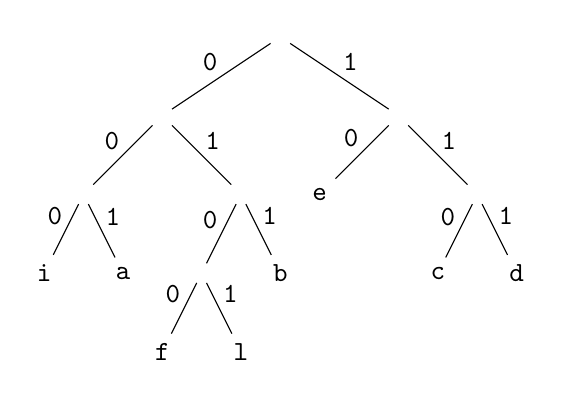
\begin{tikzpicture}[
    level distance=1cm,
    every node/.style={
    font=\ttfamily},
    level 1/.style={sibling distance=3cm},
    level 2/.style={sibling distance=2cm},
    level 3/.style={sibling distance=1cm}]
    \def\lbl#1{\ifnum#1=0 edge from parent node[draw=none,xshift=-4pt, yshift=5pt] {0}
        \else edge from parent node[draw=none, xshift=4pt, yshift=5pt] {1}\fi}

    \node {}
    child {node {}
        child {node {}
            child {node {i} \lbl{0}}
            child {node {a} \lbl{1}}
        \lbl{0}}
        child {node {}
            child {node {}
                child {node {f} \lbl{0}}
                child {node {l} \lbl{1}}
            \lbl{0}}
            child {node {b} \lbl{1}}
        \lbl{1}}
    \lbl{0}}
    child {node {}
        child {node {e} \lbl{0}}
        child {node {}
            child {node {c} \lbl{0}}
            child {node {d} \lbl{1}}
        \lbl{1}}
    \lbl{1}};
\end{tikzpicture}
\end{center}

\Q
Décoder le message suivant : 0100001110000010110.
\medskip

Quelle est la particularité de ce codage ?

\Q
On suppose l'arbre de codage connu. Les messages codés sont stockés dans des listes.
\medskip

Écrire une fonction de décodage en précisant les structures de données utilisées.

\Q
Encoder le mot \og difficile \fg{}.
\medskip

Écrire une fonction d'encodage en précisant les structures de données utilisées.

\Q
Quel est l'intérêt de ce type de codage par rapport aux codages à longueur fixe comme le code ASCII ?
\newpage

\Corrige

\Q
Le mot encodé est \og facile \fg{} : \begin{tabular}{| c | c | c | c | c | c |}
    \hline
    0100 & 001 & 110 & 000 & 0101 & 10\\
    \hline
    f & a & c & i & l & e\\
    \hline
\end{tabular}
\medskip

Nous constatons que les codes associés aux caractères n'ont pas tous la même longueur. Or, nous sommes capables de décoder un mot sans aucune ambiguïté, sans nous soucier de la longueur de chaque code. Aucun code n'est préfixe de l'autre, aucun caractère ne se trouve sur un nœud interne de l'arborescence, ils sont tous placés sur une feuille. Si l'on considère un code à longueur fixe comme le code ASCII, nous obtenons un arbre binaire complet équilibré.

\Q
On peut représenter un arbre binaire par le type :

\lstinputlisting[linerange={1-1}]{\SourceFile}

Ce qui donne l'arbre suivant pour l'exemple :

\lstinputlisting[linerange={3-16}]{\SourceFile}

Pour décoder le message, on parcourt l'arbre en lisant le message encodé caractère par caractère :

\lstinputlisting[linerange={18-29}]{\SourceFile}

\Q
Compte tenu du codage donné dans l'énoncé, le mot \og difficile \fg{} devient :
\medskip

\begin{tabular}{| c | c | c | c | c | c | c | c | c | c |}
    \hline
    d & i & f & f & i & c & i & l & e\\
    \hline
    111 & 000 & 0100 & 0100 & 000 & 110 & 000 & 0101 & 10\\
    \hline
\end{tabular}
\medskip

Une possibilité est de parcourir l'arbre et d'ajouter tous les codes à une table de hachage puis de parcourir le mot à encoder en cherchant les codes correspondants aux caractères dans la table :

\lstinputlisting[linerange={31-50}]{\SourceFile}

Ce type d'encodage est très intéressant pour la compression sans perte d'information. Dans la plupart des fichiers, le nombre d'occurrences de chaque caractère très variable : certains caractères sont plus fréquents que d'autres. Il est donc intéressant de donner aux plus fréquents les codes les plus courts afin de réduire la taille du fichier. Le code de Huffman (voir exercice sur le sujet) entre dans cette catégorie ; il est même optimal en ce qui concerne la compression par un code préfixé.
\medskip

Pour stocker de la façon la plus compacte possible un message codé avec un code préfixé, nous pouvons découper le message en morceaux de 32 bits (en admettant que les entiers sont codés sur 32 bits) et stocker les entiers correspondants dans un tableau :

\lstinputlisting[firstline=52]{\SourceFile}

\Fin
